% neural-sgdb — arXiv preprint draft.
% Compile with pdfLaTeX:  pdflatex neural-sgdb-telepathy.tex  (x2 for refs)
% arXiv submission: upload the LaTeX source (this file + the .bbl is not
% needed; thebibliography is inline). Standard article class, no exotic deps.
% Note: the demo/tool name p2p_telepathy is a code identifier; the paper uses
% scientific language ("peer-to-peer memory synchronization") throughout.
\documentclass[11pt,twocolumn]{article}

\usepackage[letterpaper,margin=0.95in]{geometry}
\usepackage{amsmath,amssymb}
\usepackage{booktabs}
\usepackage{graphicx}
\usepackage[colorlinks=true,linkcolor=blue,citecolor=blue,urlcolor=blue]{hyperref}
\usepackage{microtype}
\usepackage{tikz}
\usetikzlibrary{positioning,arrows.meta,calc,plotmarks}
\emergencystretch=2em

\newcommand{\neural}{{\sf neural-sgdb}}

\title{Memories, not Packets: A Zero-Dependency \texttt{no\_std} Memory
Substrate for AI Agents with Conflict-Preserving Peer Synchronization}

\author{Marcelo Scapin Rovani\thanks{Project: \url{https://github.com/msrovani/neural-sgdb}}
\\ \texttt{neural-os-core} community extraction (MIT OR Apache-2.0)}

\date{\today}

\begin{document}

\maketitle

\begin{abstract}
AI agents operate with ephemeral context windows: memory is lost between
turns, across instances, and after crashes. We present \neural{}, a persistent,
transferable memory database for AI agents extracted from a bare-metal
operating system, designed under strict constraints: \emph{zero external
dependencies}, dual \texttt{no\_std} + \texttt{std} operation, and
byte-identical on-disk formats shared with the parent OS. The system stores
\emph{memories}---documents with a cognitive layer ($L_0$--$L_7$), a vector
clock and an identity---rather than opaque data. Semantic recall combines
binary quantization (BQ) as a coarse candidate filter with FP32 cosine
rescore, SIMD Hamming dispatch (AVX-512/AVX2/scalar), a multi-index-hashing
(MIH) accelerator, and an optional lexical BM25-style dual path. Storage is an
append-log with per-record CRC, atomic compaction, and a byte-exact log format
(TKLV/TKCK) with checkpoint fast-mount. Peers synchronize memories through a
conflict-preserving CRDT: concurrent writes are \emph{preserved}, never
last-writer-wins-discarded, and an AI at the root of the process arbitrates the
preserved conflicts at read time using recency, importance and temporal
validity. We report measured performance (an order-of-magnitude write
throughput improvement via a persistent lazy storage handle, microsecond
recall, ~$3\times$ faster volume mounting under churn), a reproducible
two-instance peer-synchronization convergence demo (agent-to-agent memory
replication), and the honest costs of the model: eventual consistency, absence
of global ordering, and deferred conflict resolution.
\end{abstract}

\begin{center}
\textbf{Keywords:} AI-agent memory; CRDT; conflict-free replicated data types;
binary quantization; approximate nearest neighbor; \texttt{no\_std}; adaptive
radix tree; cognitive architectures
\end{center}

\section{Introduction}
\label{sec:intro}

State-of-the-art AI agents are bounded by a context window: reasoning state,
tool results and conversation are ephemeral and do not survive the session.
Recent systems address this with external memory---agentic file stores,
retrieval-augmented generation over long-term stores, and hierarchical
cognitive memories~\cite{memgpt,letta,mem0,graphiti,contextual}. Most of these
assume a central database, a network stack, and a dependency-rich runtime.

We take a different premise, inherited from a bare-metal operating system that
boots with AI: memory should be a first-class substrate that lives on the
device, survives power loss, transfers between instances, and does not require
a server. This leads to a design space rarely explored together: \emph{zero
dependencies}, \emph{\texttt{no\_std} + \texttt{std} dual mode}, \emph{format
stability across an OS boundary}, and \emph{peer-to-peer memory exchange with
conflict preservation}.

The contribution of this paper is the \neural{} system and the empirical
evidence around it:
\begin{enumerate}
  \item A memory model with 8 cognitive layers, a length-prefixed binary
        document format (NMD1) byte-identical to the parent OS, and a vector
        clock with semantic equality.
  \item A recall stack combining BQ coarse filtering, FP32 rescore, SIMD
        Hamming dispatch, auto-oversampling by dimensionality, MIH
        acceleration, and an optional lexical dual path---all format-neutral.
  \item A storage layer (CRC append-log and a byte-exact log codec) with
        checkpoint fast-mount, atomic compaction, and in-place tombstone
        invalidation.
  \item A conflict-preserving CRDT synchronization protocol (peer-to-peer
        memory exchange)\footnote{\emph{Terminology.} We use
        \emph{peer-to-peer memory synchronization} throughout; the same
        mechanism is also described---equivalently, in our view---as
        \emph{memory exchange}, \emph{gossip-style memory dissemination},
        \emph{causal memory propagation}, \emph{synchronized memory transfer},
        or \emph{agent-to-agent memory replication}. We treat these as
        synonyms; readers may use whichever they prefer.}
        with delta sending, and a principled arbitration model in which an AI
        at the root of the process resolves preserved conflicts at read time.
  \item Measured results: $\sim 38\times$ faster writes from a single storage
        optimization, microsecond recall, $\sim 2.9\times$ faster volume
        mounting under churn, and a reproducible two-instance convergence
        experiment.
\end{enumerate}

We are explicit about what we do \emph{not} claim: no linearizability, no
global ordering, and no automatic conflict resolution. These are the honest
costs of the peer-to-peer model, and we argue they are acceptable---and in some
respects preferable---for agent memory.

\begin{figure*}[t]
\centering
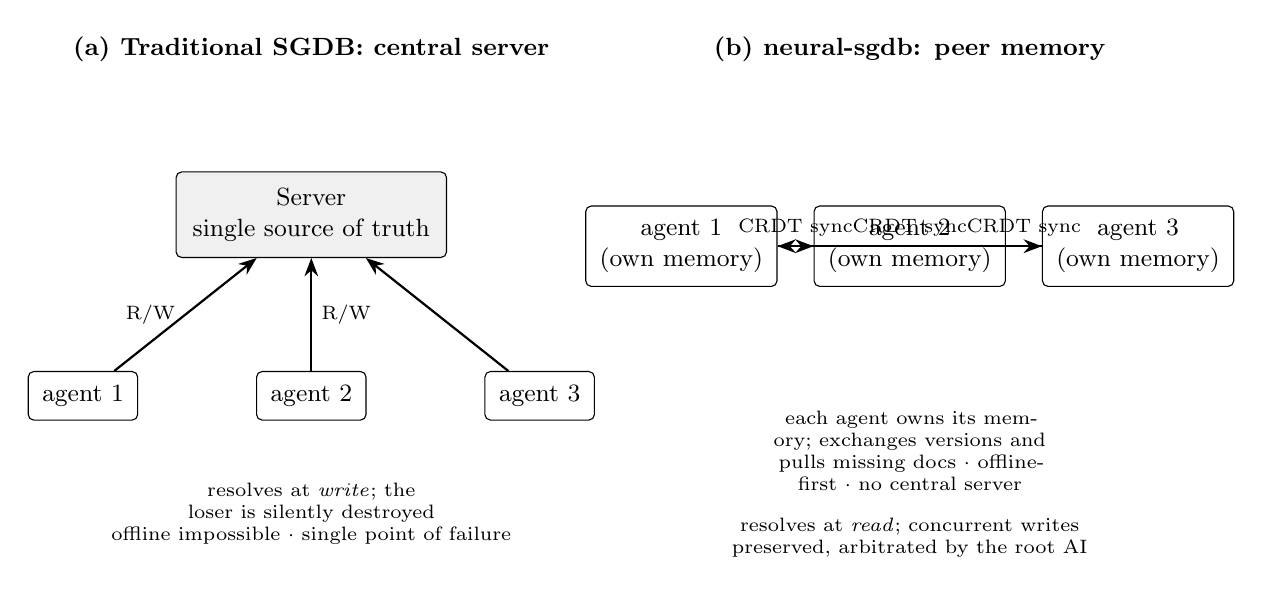
\begin{tikzpicture}[
  agent/.style={draw, rectangle, rounded corners=2pt, inner sep=5pt, align=center, font=\small},
  srv/.style={draw, rectangle, rounded corners=2pt, inner sep=6pt, align=center, font=\small, fill=gray!12},
  arrow/.style={-{Stealth}, thick},
  note/.style={font=\scriptsize, text width=5.6cm, align=center},
]
% --- traditional panel ---
\node[font=\small\bfseries] (t1) at (0,4.7) {(a) Traditional SGDB: central server};
\node[srv] (srv) at (0,2.6) {Server\\single source of truth};
\node[agent] (a1) at (-2.9,0.3) {agent 1};
\node[agent] (a2) at (0,0.3) {agent 2};
\node[agent] (a3) at (2.9,0.3) {agent 3};
\draw[arrow] (a1) -- (srv) node[midway,left,font=\scriptsize] {R/W};
\draw[arrow] (a2) -- (srv) node[midway,right,font=\scriptsize] {R/W};
\draw[arrow] (a3) -- (srv);
\node[note] (n1) at (0,-1.2) {resolves at \emph{write}; the loser is silently destroyed\\offline impossible $\cdot$ single point of failure};
% --- neural panel ---
\begin{scope}[xshift=7.6cm]
\node[font=\small\bfseries] (t2) at (0,4.7) {(b) neural-sgdb: peer memory};
\node[agent] (b1) at (-2.9,2.2) {agent 1\\(own memory)};
\node[agent] (b2) at (0,2.2) {agent 2\\(own memory)};
\node[agent] (b3) at (2.9,2.2) {agent 3\\(own memory)};
\draw[arrow] (b1) -- (b2) node[midway,above,font=\scriptsize] {CRDT sync};
\draw[arrow] (b2) -- (b3) node[midway,above,font=\scriptsize] {CRDT sync};
\draw[arrow] (b3) -- (b1) node[midway,above,font=\scriptsize] {CRDT sync};
\node[note] (n2) at (0,-0.4) {each agent owns its memory; exchanges versions and\\pulls missing docs $\cdot$ offline-first $\cdot$ no central server};
\node[note, font=\scriptsize] (n3) at (0,-1.5) {resolves at \emph{read}; concurrent writes preserved, arbitrated by the root AI};
\end{scope}
\end{tikzpicture}
\caption{Two memory architectures. (a) Traditional: agents read/write a
central server; the server resolves conflicts at write time and silently
destroys the loser; agents are unusable offline. (b) \neural{}: each agent owns
a local memory, peers synchronize causally through a conflict-preserving CRDT,
and concurrent versions survive until an arbiter resolves them at read time.}
\label{fig:comparison}
\end{figure*}

\section{Related Work}
\label{sec:related}

\paragraph{Agent memory.}
MemGPT/Letta~\cite{memgpt,letta} formalize hierarchical memory (working vs.\
archival) with paging and background consolidation; Mem0~\cite{mem0} adds
multi-signal retrieval and distillation; Zep/Graphiti~\cite{graphiti} store
temporal knowledge graphs with validity windows and provenance; Anthropic's
contextual retrieval~\cite{contextual} demonstrates large retrieval-failure
reductions by prepending chunk context and adding a lexical (BM25) path and a
reranker. We share the memory-as-substrate view and adopt the lexical dual
path and validity-window patterns, but keep zero dependencies and peer-to-peer
sync.

\paragraph{Approximate nearest neighbor.}
Sign-based binary quantization is a compact candidate generator in
production ANN systems~\cite{qdrantbq}; Qdrant reports high recall with
$2$--$4\times$ oversampling followed by full-precision rescore. Multi-index
hashing~\cite{mih} turns exact Hamming search over binary codes into a
sub-linear candidate search. ScaNN~\cite{scann} and Weaviate~\cite{weaviate}
explore anisotropic and multi-codebook quantization. We adopt oversampling and
MIH; multi-codebook quantization is future work that would require a new
opt-in encoding (our stored bit-vectors are a format contract).

\paragraph{Log-structured storage.}
Append-only logs with per-record checksums, checkpointing and
compaction~\cite{bitcask,sqlitewal} are the right family for a single-process
substrate; LSM compaction amplification~\cite{rocksdb} is unnecessary at this
scale. Our TKLV/TKCK codec follows this family and is byte-identical to the
parent OS.

\paragraph{Conflict-free replicated data types.}
CRDTs~\cite{shapiro} give eventual convergence under commutativity. Delta
state CRDTs~\cite{delta} shrink sync payloads; dotted version
vectors~\cite{dvv} compress causal metadata. Our protocol is a version-counter
CRDT with explicit conflict preservation (a multi-value register), delta
sending, and a caller-supplied clock seam (wall-clock time is never assumed by
the CRDT itself).

\section{System Design}
\label{sec:design}

\begin{figure*}[t]
\centering
\resizebox{\textwidth}{!}{%
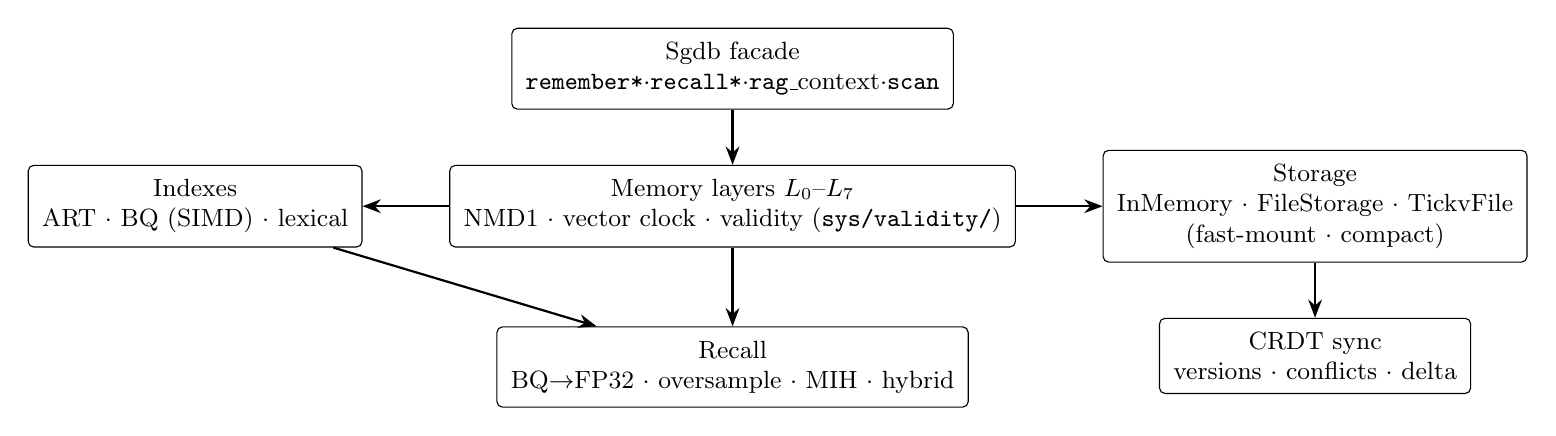
\begin{tikzpicture}[
  box/.style={draw, rounded corners=2pt, inner sep=5pt, align=center, font=\small},
  arr/.style={-{Stealth}, thick},
]
\node[box] (api) {Sgdb facade\\ \texttt{remember*}$\cdot$\texttt{recall*}$\cdot$\texttt{rag}\textunderscore context$\cdot$\texttt{scan}};
\node[box, below=7mm of api] (layers) {Memory layers $L_0$--$L_7$\\ NMD1 $\cdot$ vector clock $\cdot$ validity ($\texttt{sys/validity/}$)};
\node[box, left=11mm of layers] (idx) {Indexes\\ ART $\cdot$ BQ (SIMD) $\cdot$ lexical};
\node[box, right=11mm of layers] (stor) {Storage\\ InMemory $\cdot$ FileStorage $\cdot$ TickvFile\\ (fast-mount $\cdot$ compact)};
\node[box, below=10mm of layers] (recall) {Recall\\ BQ$\to$FP32 $\cdot$ oversample $\cdot$ MIH $\cdot$ hybrid};
\node[box, below=7mm of stor] (sync) {CRDT sync\\ versions $\cdot$ conflicts $\cdot$ delta};
\draw[arr] (api) -- (layers);
\draw[arr] (layers) -- (idx);
\draw[arr] (layers) -- (stor);
\draw[arr] (layers) -- (recall);
\draw[arr] (stor) -- (sync);
\draw[arr] (idx) -- (recall);
\end{tikzpicture}%
}
\caption{Architecture of \neural{}. The \texttt{Sgdb} facade exposes
\emph{memories, not data}: documents with a layer, a vector clock and a
validity window. Derived indexes (ART, BQ, lexical) and pluggable storage are
seams; peer synchronization rides on the storage layer. All components compile
to \texttt{no\_std} (only \texttt{alloc}) with zero external dependencies.}
\label{fig:arch}
\end{figure*}

\subsection{Memory model and format}
\label{sec:model}

A memory document carries a layer $L \in \{L_0,\dots,L_7\}$ (sensory, working,
episodic short/long, semantic, procedural, reserved, identity), a key, a
vector clock, a payload, and an optional packed binary embedding. The NMD1
encoding is length-prefixed and byte-identical to the parent OS; golden byte
tests pin the layout. A zero-copy view allows payload access without full
deserialization.

Layers $L_0$/$L_1$ live in RAM and flush to storage at an explicit
checkpoint; $L_2$--$L_7$ persist immediately. Semantic memories ($L_4$/$L_5$)
store the caller-supplied embedding payload and a 1-bit quantized bit-vector
$\operatorname{sign}(x)>0$; the textual companion lives in $L_2$.

\subsection{Recall}
\label{sec:recall}

Recall follows a Qdrant-style coarse-to-fine pipeline:
\begin{equation}
\textit{recall}(q,k) = \operatorname{top}_k\!\big(
  \operatorname{rescore}_{\mathrm{FP32}}\big(
    \operatorname{top}_{k\cdot s}(\mathrm{BQ}(q))\big)\big),
\label{eq:recall}
\end{equation}
where the Hamming distance uses SIMD dispatch
($\mathsf{AVX\text{-}512} > \mathsf{AVX2} > \mathsf{scalar}$, selected at
runtime via \texttt{cpu\_caps()}) and the oversampling factor $s$ is chosen
automatically by dimensionality (1 word $\to 16$, 2--4 words $\to 8$, else
$4$) because 1-bit BQ degrades below $\sim$768 dimensions. A bounded
max-heap keeps top-$k$ ranking $O(N\cdot D/64 + N\log k)$.

Two accelerators are format-neutral: \emph{MIH} partitions each stored
bit-vector into blocks, indexes block hashes, and probes the query blocks to
recover sub-linear candidate sets~\cite{mih}; and a \emph{lexical} BM25-style
inverted index over $L_2$/$L_3$ texts implements the dual-path pattern of
contextual retrieval~\cite{contextual}, merged with semantic hits in
\texttt{recall\_hybrid}. Ranking may be weighted by recency (from a
wall-clock timestamp embedded in the key), importance (from the layer), and
semantic distance.

\begin{figure*}[t]
\centering
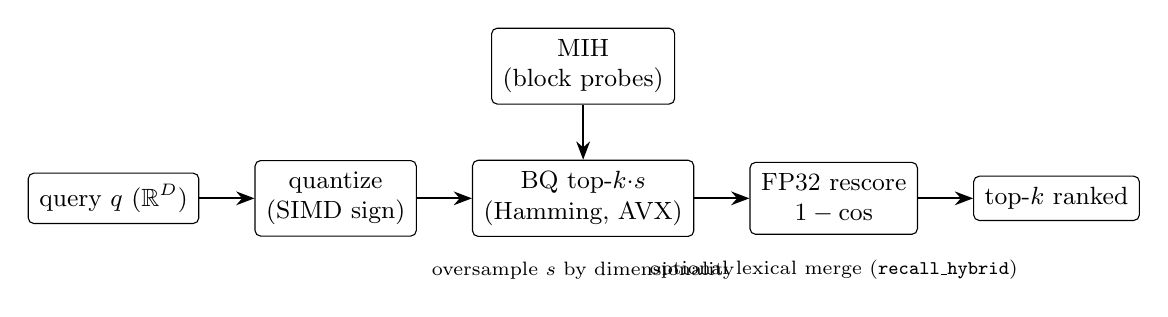
\begin{tikzpicture}[
  box/.style={draw, rounded corners=2pt, inner sep=4pt, align=center, font=\small},
  arr/.style={-{Stealth}, thick},
]
\node[box] (q) {query $q$ ($\mathbb{R}^D$)};
\node[box, right=7mm of q] (qk) {quantize\\ (SIMD sign)};
\node[box, right=7mm of qk] (bq) {BQ top-$k{\cdot}s$\\ (Hamming, AVX)};
\node[box, above=7mm of bq] (mih) {MIH\\ (block probes)};
\node[box, right=7mm of bq] (fp) {FP32 rescore\\ $1-\cos$};
\node[box, right=7mm of fp] (out) {top-$k$ ranked};
\draw[arr] (q) -- (qk);
\draw[arr] (qk) -- (bq);
\draw[arr] (mih) -- (bq);
\draw[arr] (bq) -- (fp);
\draw[arr] (fp) -- (out);
\node[font=\scriptsize, below=2mm of bq] {oversample $s$ by dimensionality};
\node[font=\scriptsize, below=2mm of fp] {optional lexical merge (\texttt{recall\_hybrid})};
\end{tikzpicture}
\caption{Coarse-to-fine recall (Eq.~\ref{eq:recall}). A coarse binary-quantized
Hamming filter (SIMD-dispatched, optionally accelerated by multi-index hashing)
retrieves an oversampled candidate pool; full-precision cosine rescore re-ranks
it. All stages are format-neutral---stored bit-vectors never change.}
\label{fig:recall}
\end{figure*}

\subsection{Storage}
\label{sec:storage}

Backends implement a four-method \texttt{Storage} trait. \texttt{FileStorage}
is a CRC-protected append-log with atomic compaction; \texttt{TickvFile} is
the byte-exact TKLV codec of the parent OS, with a TKCK checkpoint record
enabling \emph{fast-mount} (header-only scan, FNV index verification, per-entry
stale check) with a full-scan fallback, and in-place tombstone invalidation
($\texttt{magic}[3]{=}0$) before overwrite---making dead space
header-detectable. A single measured optimization, a persistent lazy append
handle, reduced write latency by $\sim 38\times$ (Section~\ref{sec:eval}).

\subsection{Peer-to-Peer Memory Synchronization}
\label{sec:sync}

Each node pairs an \texttt{Sgdb} instance with a \texttt{CrdtMemorySync}
holding its own version counter, a count of independent local writes
(\texttt{own\_writes}), the versions known of peers, and a preserved conflict
set. The merge is a multi-value register with explicit verdicts:
self-packets ignored, stale/duplicate versions rejected (no regression), new
versions adopted when no conflicting local state exists, and \emph{concurrent}
versions preserved in the conflict set. Delta sending
(\S\ref{sec:sync}) ships only versions a peer has not seen---gossip-style
dissemination of the causal state rather than the full history.

Exchanging versions is the causal trigger; transferring documents (memory
transfer) is a diff-pull: a peer that learns another advanced replicates the
missing docs (\texttt{get} $\to$ \texttt{put}). Two instances converge with no
central server. Because resolution writes are themselves causal CRDT writes,
arbitration outcomes propagate to every peer via the same dissemination
mechanism.

\begin{figure*}[t]
\centering
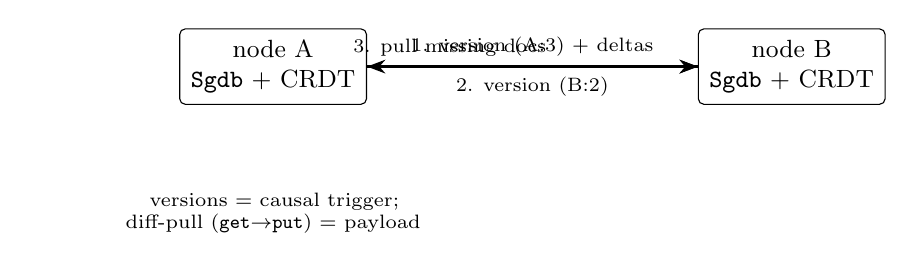
\begin{tikzpicture}[
  box/.style={draw, rounded corners=2pt, inner sep=4pt, align=center, font=\small},
  arr/.style={-{Stealth}, thick},
  tline/.style={font=\scriptsize},
]
\node[box] (a) {node A\\ \texttt{Sgdb} + CRDT};
\node[box, right=42mm of a] (b) {node B\\ \texttt{Sgdb} + CRDT};
\draw[arr] (a) -- node[tline, above] {1. version (A:3) $+$ deltas} (b);
\draw[arr] (b) -- node[tline, below] {2. version (B:2)} (a);
\draw[arr, dashed] (a) -- node[tline, above, pos=0.25] {3. pull missing docs} (b);
\node[font=\scriptsize, below=10mm of a, text width=6cm, align=center] {versions = causal trigger;\\ diff-pull (\texttt{get}$\to$\texttt{put}) = payload};
\end{tikzpicture}
\caption{Peer-to-peer memory exchange between two instances. Versions (and
deltas) are the causal trigger; the pull phase replicates only the documents a
peer is missing. The merge preserves concurrent writes (multi-value) instead of
discarding them.}
\label{fig:sync}
\end{figure*}

\subsection{Arbitration by an AI at the root}
\label{sec:arbitration}

Because concurrent writes are preserved rather than resolved, the system
defers semantic decisions to the layer that has the full context: an AI at the
root of the process (in the parent OS, running from boot). Arbitration is a
five-step pipeline: \emph{harvest} the preserved conflict set (complete
information is guaranteed---no update was destroyed); \emph{contextualize}
along the causal chain using episodic memories; \emph{weigh} recency (wall
clock in the key), importance (layer) and behavioral consistency; \emph{decide}
via one of four policies---deterministic recency-first ranking at read time,
temporal validity invalidation (invalidate-not-delete), semantic fusion
(write a unified document and \texttt{supersede} the originals), or escalation
to a human/agent; and \emph{propagate} the resolution as a new causal write.

This contrasts with the traditional resolve-at-write model, where a central
server silently destroys the losing version. Here arbitration runs on complete
data, at any time, and the verdict is CRDT state that converges across peers.

\begin{figure*}[t]
\centering
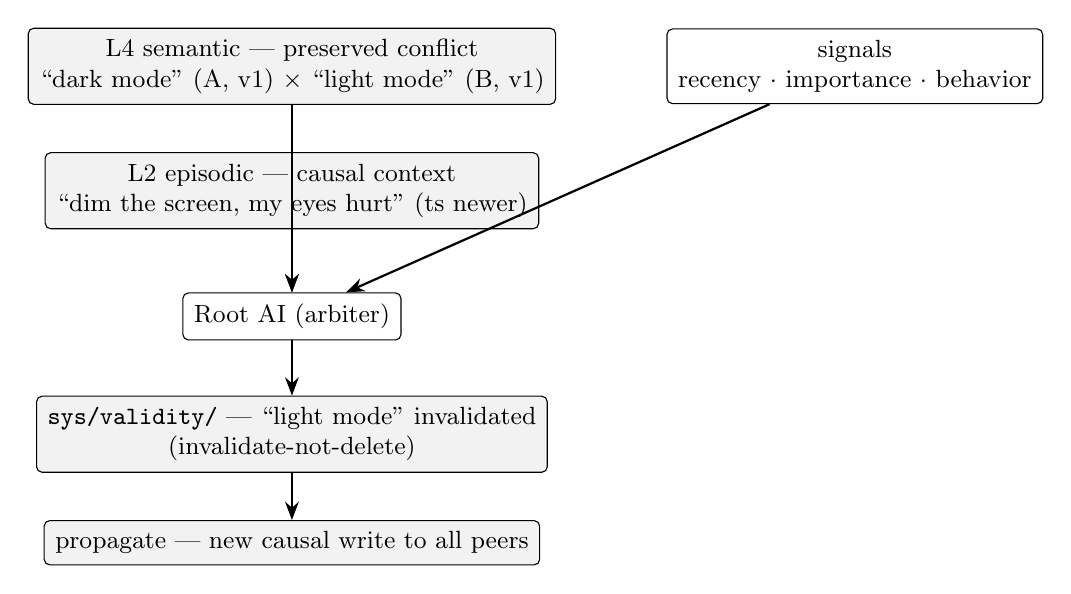
\begin{tikzpicture}[
  box/.style={draw, rounded corners=2pt, inner sep=4pt, align=center, font=\small},
  layer/.style={draw, rounded corners=2pt, inner sep=4pt, align=center, font=\small, fill=gray!10},
  arr/.style={-{Stealth}, thick},
]
\node[layer] (l4) {L4 semantic --- preserved conflict\\ ``dark mode'' (A, v1) $\times$ ``light mode'' (B, v1)};
\node[layer, below=6mm of l4] (l2) {L2 episodic --- causal context\\ ``dim the screen, my eyes hurt'' (ts newer)};
\node[box, right=14mm of l4] (sig) {signals\\ recency $\cdot$ importance $\cdot$ behavior};
\node[box, below=8mm of l2] (root) {Root AI (arbiter)};
\node[layer, below=7mm of root] (val) {$\texttt{sys/validity/}$ --- ``light mode'' invalidated\\ (invalidate-not-delete)};
\node[layer, below=6mm of val] (prop) {propagate --- new causal write to all peers};
\draw[arr] (l4) -- (root);
\draw[arr] (l2) -- (root);
\draw[arr] (sig) -- (root);
\draw[arr] (root) -- (val);
\draw[arr] (val) -- (prop);
\end{tikzpicture}
\caption{Layered arbitration of a preserved conflict (\S\ref{sec:arbitration}).
The root AI combines the two concurrent L4 versions with the causal L2
context and a recency/importance/behavior signal, then materializes the verdict
as a validity window---an invalidation that is itself a new causal write and
propagates to every peer.}
\label{fig:arbitration}
\end{figure*}

\section{Design Rationale}
\label{sec:rationale}

Four constraints shape the system, and each has a concrete consequence:

\begin{itemize}
  \item \textbf{Zero external dependencies.} The substrate is meant to run
        inside an operating system and to be audited line by line. Every
        algorithm---ART, BQ/Hamming, CRC32, FNV, BM25, CRDT---is implemented
        in-crate. This is a deliberate cost: no reuse of mature libraries, in
        exchange for portability and a small trusted-computing base.
  \item \textbf{Dual \texttt{no\_std} + \texttt{std}.} The core is
        \texttt{no\_std} (only \texttt{alloc}); storage backends and the UDP
        demo transport are \texttt{std}-gated features. The same code runs on
        bare metal and on the host, enforced by a CI gate
        (\texttt{cargo check --no-default-features --target
        x86\_64-unknown-none}).
  \item \textbf{Byte-identical formats.} NMD1 (documents) and TKLV/TKCK
        (storage) are contracts shared with the parent OS: golden byte tests
        pin the layout, and a volume written by either side mounts on the
        other. Format changes therefore require synchronized change on both
        sides---new capabilities are introduced as new opt-in encodings or
        side indices, never by mutating existing bytes.
  \item \textbf{Seams, not globals.} There is no global engine: the clock is a
        \texttt{now: u64} parameter, SIMD capability is injected via
        \texttt{cpu\_caps()}/\texttt{set\_cpu\_caps()}, and storage is the
        four-method \texttt{Storage} trait. This keeps the substrate testable
        and embeddable in a kernel.
\end{itemize}

We also deliberately chose an append-log with checkpoints over an
LSM~\cite{rocksdb}: at this scale (thousands to millions of small memories on a
single device), write/read amplification from compaction is pure cost, while a
CRC-protected append-log with an atomic compact and a TKCK fast-mount gives
power-loss safety with a fraction of the machinery.

\section{Evaluation}
\label{sec:eval}

All measurements are from the project's benchmark/stress harnesses on a
consumer laptop (AVX2; no AVX-512). The test suite is $92{+}1$ unit/doc tests
(default features) and $102{+}1$ with the \texttt{p2p} feature; the
\texttt{no\_std} gate
(\texttt{cargo check --no-default-features --target x86\_64-unknown-none})
is clean.

\subsection{Storage write path}
\label{sec:eval-storage}

Replacing a per-write file open/close with a persistent lazy append handle
reduced raw \texttt{put} latency from $185\,\mu$s to $4.8\,\mu$s
($\sim 38\times$), and end-to-end semantic writes from $422\,\mu$s to
$22\,\mu$s ($\sim 19\times$). A crash-invariant test verifies that writes after
atomic compaction target the new file (never a stale inode/file object).

\begin{figure*}[t]
\centering
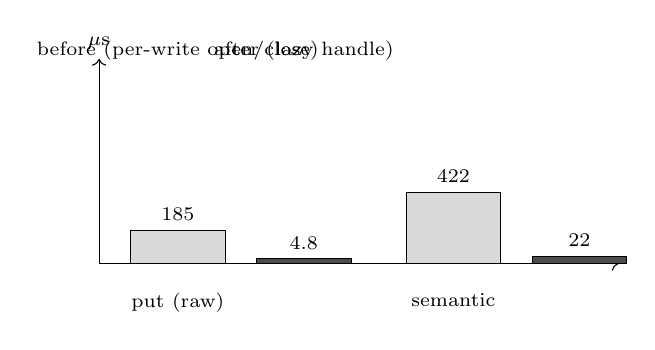
\begin{tikzpicture}[
  bar/.style={fill=gray!30, draw},
  bar2/.style={fill=black!70, draw},
  lb/.style={font=\scriptsize},
]
\draw[->] (0,0) -- (0,2.6) node[above,lb] {$\mu$s};
\draw[->] (0,0) -- (6.6,0);
% raw put: 185 -> 4.8
\draw[bar] (0.4,0) rectangle (1.6,0.42); \node[lb, above] at (1.0,0.42) {185};
\draw[bar2] (2.0,0) rectangle (3.2,0.06); \node[lb, above] at (2.6,0.06) {4.8};
\node[lb, below] at (1.0,-0.25) {put (raw)};
% remember_semantic: 422 -> 22
\draw[bar] (3.9,0) rectangle (5.1,0.9); \node[lb, above] at (4.5,0.9) {422};
\draw[bar2] (5.5,0) rectangle (6.7,0.09); \node[lb, above] at (6.1,0.09) {22};
\node[lb, below] at (4.5,-0.25) {semantic};
\node[lb, at={(1.0,2.7)}] {before (per-write open/close)};
\node[lb, at={(2.6,2.7)}] {after (lazy handle)};
\end{tikzpicture}
\caption{Write latency before and after the persistent lazy append handle:
raw \texttt{put} $185\to4.8\,\mu$s ($\sim 38\times$) and end-to-end semantic
writes $422\to22\,\mu$s ($\sim 19\times$). Bars are to the same scale; values
annotated.}
\label{fig:writes}
\end{figure*}

\subsection{Recall}
\label{sec:eval-recall}

BQ top-5 over 10\,000 vectors $\times$ 1024 dimensions dropped from
$213\,\mu$s to $160\,\mu$s/query after removing a locked atomic RMW from the
per-call Hamming dispatch ($\sim 25\%$). On a correlated-cluster corpus, the
coarse BQ filter alone recovers $22\%$ of the exact FP32 top-5 at
oversample $1\times$, rising to $35\%$ at $16\times$---consistent with the
known property that sign-BQ separates the \emph{cluster} but not the
\emph{exact member}; the FP32 rescore then re-ranks the candidates. With
16-dimension embeddings, low-dimensional bit collision drops exact@1 to
$\sim 42\%$; raising the candidate pool via oversampling restores it.

\begin{figure*}[t]
\centering
\begin{tikzpicture}[lb/.style={font=\scriptsize},plot/.style={-{Stealth}}]
\draw[->] (0,0) -- (0,3.0) node[above,lb] {recall@5 (\%)};
\draw[->] (0,0) -- (5.4,0) node[right,lb] {oversample $s$};
\foreach \x/\y/\lab in {1/0.66/22,2/0.66/22,4/0.72/24,8/0.9/30,16/1.05/35}{
  \fill (\x,0) circle (1pt);
  \fill (\x,\y) circle (1.5pt);
  \node[lb, above] at (\x,\y) {\lab};
  \node[lb, below] at (\x,0) {\x};
}
\draw[black, thick] (1,0.66) -- (2,0.66) -- (4,0.72) -- (8,0.9) -- (16,1.05);
\end{tikzpicture}
\caption{Coarse BQ candidate recall@5 vs.\ oversample on a correlated
1024-dimension cluster corpus. The coarse filter separates the cluster but not
the exact member; enlarging the candidate pool raises recall
($22\%$ at $1\times$ to $35\%$ at $16\times$), and the FP32 rescore then
re-ranks the candidates.}
\label{fig:oversample}
\end{figure*}

\subsection{Fast-mount under churn}
\label{sec:eval-mount}

On a churned volume (35\,000 records, 5\,000 live), checkpoint fast-mount took
$14.8\,\mathrm{ms}$ vs.\ $43.2\,\mathrm{ms}$ for a full scan
($\sim 2.9\times$). On an all-live volume both read the same bytes and are at
parity; the win is not re-processing tombstones/dead records.

\begin{figure*}[t]
\centering
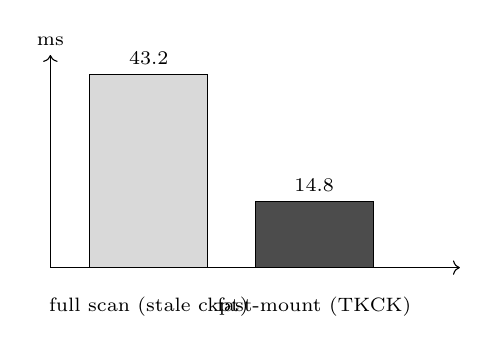
\begin{tikzpicture}[bar/.style={fill=gray!30,draw},bar2/.style={fill=black!70,draw},lb/.style={font=\scriptsize}]
\draw[->] (0,0) -- (0,2.7) node[above,lb] {ms};
\draw[->] (0,0) -- (5.2,0);
\draw[bar] (0.5,0) rectangle (2.0,2.45); \node[lb, above] at (1.25,2.45) {43.2};
\draw[bar2] (2.6,0) rectangle (4.1,0.84); \node[lb, above] at (3.35,0.84) {14.8};
\node[lb, below] at (1.25,-0.25) {full scan (stale ckpt)};
\node[lb, below] at (3.35,-0.25) {fast-mount (TKCK)};
\end{tikzpicture}
\caption{Volume mount on a churned store (35\,000 records, 5\,000 live):
full scan $43.2\,\mathrm{ms}$ vs.\ TKCK fast-mount $14.8\,\mathrm{ms}$
($\sim 2.9\times$). The checkpoint index skips tombstones/dead records.}
\label{fig:mount}
\end{figure*}

\subsection{Peer Synchronization Convergence}
\label{sec:eval-sync}
The two-instance synchronization experiment (the \texttt{p2p\_telepathy}
example) runs two \texttt{Sgdb} instances over an
in-memory transport: A writes $m_1$, B writes $m_2$; one synchronization round
replicates two documents in each direction and logs both concurrent writes as
preserved conflicts; a second round is idempotent; a reply $m_3$ propagates
back in a third round. Both instances converge to identical memory sets and
cross-recall each other's memories semantically. Convergence is idempotent and
requires no central coordinator.

\section{Discussion and Limitations}
\label{sec:discussion}

\paragraph{Eventual consistency.}
Peers diverge during the window between a write and a synchronization round.
Convergence is guaranteed (the merge is commutative, associative, idempotent,
and monotonic) but not time-bounded. For agent memory this is a feature---an
agent's memory is local and survives disconnection---but applications requiring
linearizable reads must add their own coordination.

\paragraph{No global ordering.}
There is no global sequence; the CRDT provides causal order only, and
wall-clock time must be supplied by the caller. ``Latest'' queries therefore
require a caller clock (as in our weighted ranking).

\paragraph{Deferred conflict resolution.}
Conflicts are preserved, not resolved, by design. Resolving them requires a
policy in the consuming layer; we provide primitives (weighted ranking,
validity windows, supersede) and an arbitration model, but the semantic
judgment is not automated by the substrate.

\paragraph{Other limitations.}
The demo transport is unauthenticated (production requires a signed transport);
the system is single-threaded by design; ARM SIMD (NEON) and multi-codebook
quantization are future work; the MCP embedding is a demo trigram hash, not a
real semantic model.

\subsection{Threats to validity}
\label{sec:validity}

\paragraph{Measurement.}
All numbers come from the project's benchmark harness on a single consumer
laptop (AVX2, no AVX-512), not a controlled experimental protocol. Relative
comparisons (before/after) are robust; absolute figures may not transfer.
\paragraph{Embeddings.}
Synthetic embeddings (LCG, trigram hash, cluster+noise) approximate, but do
not reproduce, production model embeddings; the BQ trade-off curve may shift
with real distributions.
\paragraph{Networking.}
The convergence experiment runs over an in-memory transport; real networks
(ordering, loss, latency) are not exercised.
\paragraph{Concurrency.}
The substrate is single-threaded by design; no multi-threaded throughput or
consistency results are reported.

\section{A Case Study: an Agent Memory Lifecycle}
\label{sec:casestudy}

We sketch one complete agent scenario to tie the pieces together.

\textbf{Turn.} The agent answers a user query; \texttt{remember\_exchange}
stores the exchange in $L_1$/$L_2$ (RAM), and \texttt{remember\_semantic}
indexes the summary in $L_4$ with a caller-supplied embedding.

\textbf{Recall.} On the next query, the embedding is run through the
coarse-to-fine pipeline (Eq.~\ref{eq:recall}): auto-oversampling widens the BQ
pool, \texttt{recall\_weighted} re-ranks by recency (from the \texttt{ts} key),
importance (layer) and semantic distance.

\textbf{Consolidation (future).} A background pass distills episodic $L_2$ into
a semantic $L_4$ fact, written as a new causal document---the substrate
"dreams" without dropping the episode.

\textbf{Transfer.} A second instance of the agent meets the first; the
peer-synchronization protocol (\S\ref{sec:sync}) exchanges versions and pulls
missing memories. Both converge; neither needed a server.

\textbf{Arbitration.} The two instances had concurrently recorded different
preferences; the conflict is preserved. The root AI (Fig.~\ref{fig:arbitration})
combines the L4 conflict with the L2 causal context and a newer timestamp,
and invalidates the stale value via \texttt{sys/validity/}---an
invalidate-not-delete that propagates to every peer.

\textbf{Forgetting.} A stale fact whose validity window has passed no longer
surfaces in \texttt{recall\_at}, while its history remains auditably intact.

\section{Reproducibility}
\label{sec:repro}

Source, tests and harnesses are public:
\url{https://github.com/msrovani/neural-sgdb}. Key commands:
\texttt{cargo test} (unit), \texttt{cargo test --features p2p},
\texttt{cargo check --no-default-features --target x86\_64-unknown-none}
(\texttt{no\_std} gate), \texttt{cargo run --release --example bench},
\texttt{cargo run --release --example stress}, and \texttt{cargo run --release
--example p2p\_telepathy --features p2p} (two-instance synchronization
experiment).

\section{Future Work}
\label{sec:future}

Planned directions include background consolidation (``dreaming'') that
distills episodic memories into semantic facts as new causal writes;
arbitration over validity windows in the sync layer; a signed/authenticated
transport; NEON SIMD; and multi-codebook quantization as an opt-in encoding
that preserves existing stored vectors.

\begin{thebibliography}{99}

\bibitem{memgpt} C.~Packer, V.~Fang, S.~Patil, K.~Lin, S.~Wooders, J.~Gonzalez.
``MemGPT: Towards LLMs as Operating Systems,'' \emph{arXiv:2310.08560}, 2023.

\bibitem{letta} Letta project. ``Letta: Stateful agents framework.''
\url{https://docs.letta.com}.

\bibitem{mem0} Mem0 project. ``The memory layer for personalized AI.''
\url{https://mem0.ai}.

\bibitem{graphiti} Zep/Graphiti. ``Zep: Temporal Knowledge Graph Architecture
for Agent Memory,'' \emph{arXiv:2501.13956}, 2025.

\bibitem{contextual} Anthropic. ``Introducing Contextual Retrieval,'' 2024.
\url{https://www.anthropic.com/news/contextual-retrieval}.

\bibitem{qdrantbq} Qdrant. ``Binary Quantization.'' \url{https://qdrant.tech}.

\bibitem{mih} M.~Norouzi, A.~Punjani, D.~Fleet. ``Fast Exact Search in Hamming
Space with Multi-Index Hashing,'' \emph{IEEE TPAMI} 36(6), 2014.

\bibitem{scann} R.~Guo et al. ``Accelerating Large-Scale Inference with
Anisotropic Vector Quantization,'' \emph{ICML}, 2020.

\bibitem{weaviate} Weaviate. ``Vector index: HFresh/SPFresh and dynamic
\emph{ef}.'', \url{https://weaviate.io}.

\bibitem{bitcask} Basho. ``Bitcask: A Log-Structured Hash Table for Fast
Key/Value Data,'' 2010.

\bibitem{sqlitewal} SQLite. ``Write-Ahead Logging.''
\url{https://sqlite.org/wal.html}.

\bibitem{rocksdb} RocksDB. ``Overview of Architecture.''
\url{https://github.com/facebook/rocksdb}.

\bibitem{shapiro} M.~Shapiro et al. ``A Comprehensive Study of Convergent and
Commutative Replicated Data Types,'' \emph{RR-7506, INRIA}, 2011.

\bibitem{delta} C.~Almeida, A.~Shoker, C.~Baquero. ``Delta State Replicated
Data Types,'' \emph{arXiv:1603.01529}, 2016.

\bibitem{dvv} N.~Pregui\c{c}a et al. ``Dotted Version Vectors: Efficient
Causality Tracking for Distributed Systems,'' \emph{OPODIS}, 2010.

\bibitem{art} V.~Leis, A.~Kemper, T.~Neumann. ``The Adaptive Radix Tree:
ARTful Indexing for Main-Memory Databases,'' \emph{DaMoN}, 2013.

\bibitem{coala} S.~Sumers, T.~Yao, K.~Narasimhan, T.~Griffiths. ``Cognitive
Architectures for Language Agents,'' \emph{TMLR}, 2024.

\end{thebibliography}

\appendix
\section{Peer-synchronization experiment trace}
\label{app:trace}

The two-instance synchronization experiment
(\texttt{cargo run --release --example p2p\_telepathy --features p2p}) prints
the following trace; concurrent writes are reported as preserved conflicts.

{\scriptsize
\begin{verbatim}
[A] lembra m1  (versão A = 1)
[B] lembra m2  (versão B = 1)
CRDT sync: node=2 v=1 CONFLITO preservado (concorrente)
CRDT sync: node=1 v=1 CONFLITO preservado (concorrente)
[↔] ronda 1: A→B 2 doc(s), B→A 2 doc(s)
[↔] ronda 2: A→B 0 doc(s)
[B] lembra m3  (versão B = 2)
[↔] ronda 3: A→B 0 doc(s), B→A 2 doc(s)
[✓] A conhece 6 docs, B conhece 6 docs
[B] recall da memória de A: ["eu sou a instancia A..."]
\end{verbatim}
}

Both instances converge to the same memory set (three memories $\times$ L2
text + L4 embedding = six documents) and cross-recall each other's memories
semantically. Round 2 is idempotent. The resolution of a later conflict (a new
causal write, e.g.\ a validity invalidation) propagates through the same
mechanism.

\end{document}
